\section{Planning That Survives Location Uncertainty}
\label{sec:planning}

Section~\ref{sec:dem} says we cannot reliably name the street that ponds first. Planning is still
possible, because the quantities that drive a plan are not the quantity that fails. Every
intervention below is evaluated the same way. Modify the terrain, re-simulate the design storm at
100\,mm over 24\,h, and measure flooding on built-up cells, \emph{excluding} the intervention's own
cells from both the before and the after mask. Moving water onto a drain does not count as removing
it. The excluded fraction is reported and stays below a few percent of built cells.

\subsection{A storm drain spiderweb routed on the real street graph}
Sparse worst-basin-to-nearest-outfall canals are how our earlier planner worked, and anecdotally
how much real retrofitting works. Two to five least-cost corridors over the elevation grid cut
20.8\,\% of street flooding in Patna and 25.7\,\% in Bengaluru. Preferring road cells and avoiding
buildings \emph{improved} the Bengaluru cut threefold, which is a useful fact on its own. Streets
trace drainage valleys in dense terrain, so buildability and hydraulics point the same way.

Scaling that idea up, we route a dense network on the actual street graph. The area's
OpenStreetMap roads \cite{osm} form a graph whose nodes carry elevations, with 42.8\,k nodes and
6.8\,k ways for Patna. Edge cost is street length plus an uphill penalty of 2\,400\,m per metre of
climb. One reverse multi-source Dijkstra search from all outfalls labels every street with its
gravity-cheapest exit. About 40 inlets are placed at the deepest cell of each flood basin, and
their exit chains trace out a forest with shared trunks that accumulate flow.

The outfalls encode a safety principle. \emph{Never the river}, because during a flood the river
runs high and a drain into it runs backwards. Instead we use the lowest \emph{safe} ground, meaning
non-built land buffered away from buildings and from the river corridor, plus downhill exits from
the domain and detention pits. Pits are handicapped by 2\,km of equivalent cost so that carrying
water away wins wherever gravity allows it. The chosen streets are then carved into the elevation
as 2\,m channels with strictly descending beds, shared trunks take the deepest bed, and the storm is
re-simulated.

\begin{table}[!t]
\centering
\caption{Measured intervention ladder for Patna at 100\,mm, all re-simulated. Costs use indicative
Indian civil-works rates of \rupee9\,000 per metre of drain, \rupee300 per m$^3$ of excavation and
\rupee6\,000 per m$^3$ of concrete storage. The dense street-routed network beats sparse canals on
\emph{both} axes.}
\label{tab:ladder}
\begin{tabular}{lccc}
\toprule
intervention & cut & flood removed & cost per m$^3$ \\
\midrule
excavation, 8 sites            & 4.1\,\%  & 0.06\,M\,m$^3$ & \rupee758 \\
detention pits only, 8 sites   & 7.8\,\%  & 0.11\,M\,m$^3$ & n/a \\
sparse canals and pits, 3.2\,km & 20.2 to 20.8\,\% & 0.28\,M\,m$^3$ & \rupee1\,309 \\
\textbf{spiderweb, 40 inlets, 44.5\,km} & \textbf{80.9\,\%} & \textbf{0.87\,M\,m$^3$} & \textbf{\rupee850} \\
distributed storage, 727 basins & 30\,\% & 0.43\,M\,m$^3$ & \rupee9\,200 \\
\bottomrule
\end{tabular}
\end{table}

\begin{figure}[!t]
\centering
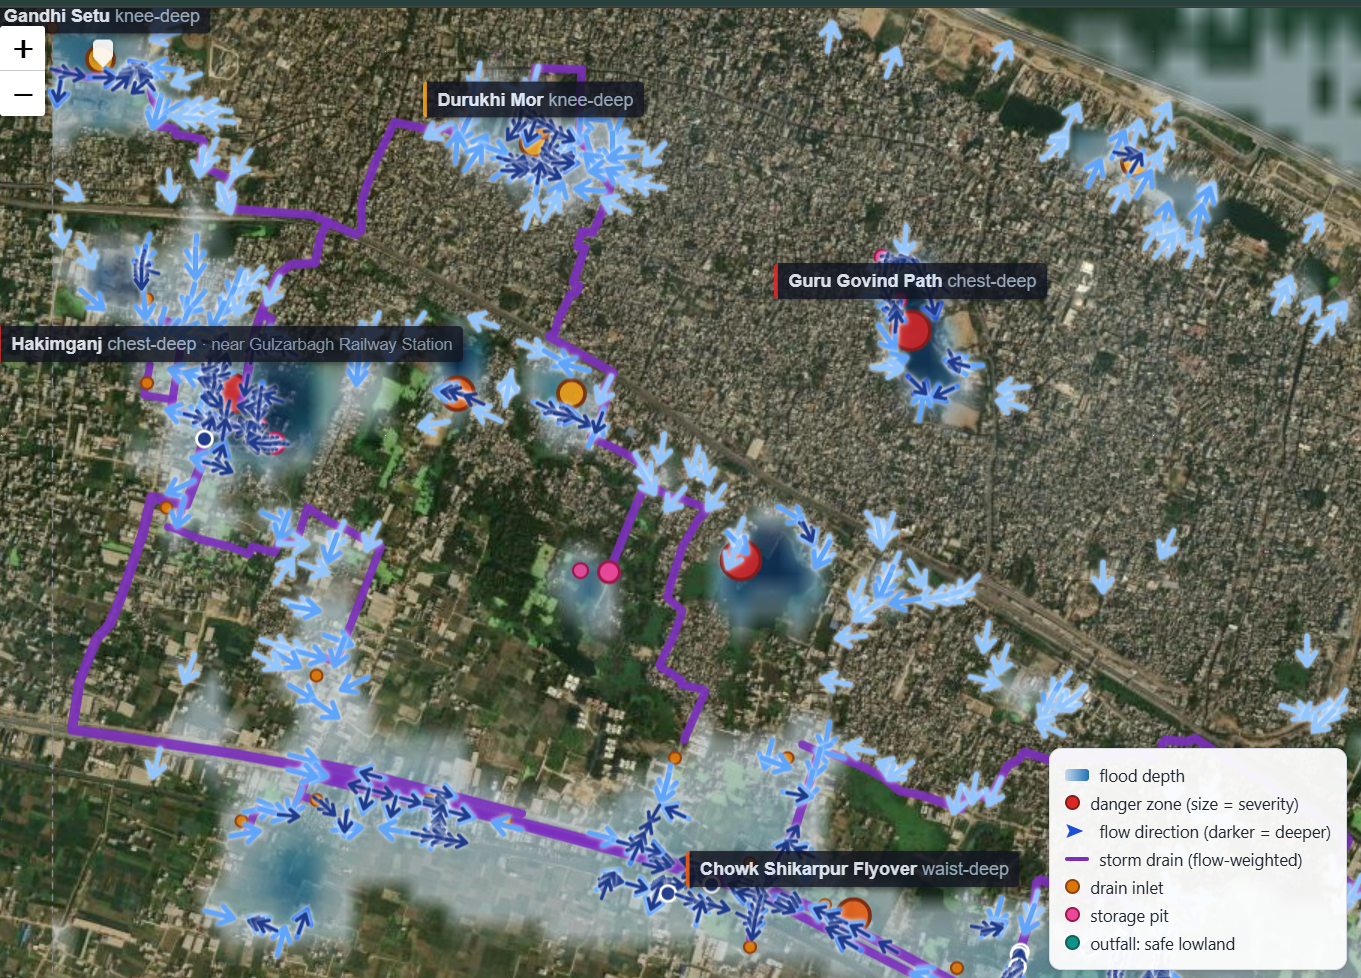
\includegraphics[width=0.99\linewidth]{figures/live_patna_sat.png}
\caption{The designed drain network over satellite imagery for eastern Patna. Purple lines are the
planned trunks, orange circles are inlets, and the arrows are the simulated flow field. The labels
are real road names carrying a predicted depth in words. The network is not drawn by hand. It is
the union of gravity-cheapest exit paths from 40 basin inlets to safe outfalls.}
\label{fig:patnasat}
\end{figure}

\textbf{Results.} Across the eight built areas the spiderweb cuts street flooding by 80.9\,\% in
Patna, 89.4\,\% in Patna-East, 80.3\,\% in Patna-West, 72.6\,\% in Bengaluru, and 63.0, 50.2, 39.2
and 32.5\,\% on the Mumbai South, East, West and North tiles, against 21 to 26\,\% for the sparse
plans. Dose-response over 25 to 200\,mm is monotone.

Density improves the \emph{economics} as well as the effectiveness. Patna costs \rupee850 per cubic
metre removed against \rupee1\,309 for the sparse plan, and Bengaluru costs \rupee1\,121, because
shared trunks spread their length across many basins. The lower Mumbai cuts are informative rather
than disappointing. Those tiles are four times larger, far denser and partly harbour, so a fixed
budget of about 40 inlets covers a smaller share of the flooding.

\subsection{Buildable and phased distributed storage}
The storage planner answers a different question. How many detention tanks, and where, to cut the
flood by a target percentage? Candidate cells are the dynamic local minima of the simulated flood,
ranked by pooled depth. Each site is sized to the water it actually holds, and the cut is
re-measured by simulation rather than assumed.

The important word is buildable. Building footprints and permanent water are excluded from
candidacy, because you cannot dig a tank under an occupied house or in the harbour. Under-street
detention stays allowed, which mirrors how Indian cities actually retrofit. Buildability is not
free on flats. Excluding building-footprint minima removes some of the deepest candidates and the
reachable ladder drops accordingly. We report that rather than quietly siting tanks inside houses.

Each area ships an explicit ranked site list of up to 1\,500 sites with coordinates, per-site
volume and an under-street flag, where 63 to 87\,\% of sites land under streets, together with a
phase ladder costed at indicative rates. Patna reaches a measured 10\,\% cut with 193 sites at
about \rupee165 crore. Mumbai-West needs 493 sites and about \rupee825 crore for the same 10\,\%.
Dense tiles reach 10\,\% and no further, which is an honest ladder rather than an aspirational one.

The planner has never seen a flood report or a news archive. Its top-ranked sites nonetheless land
on each city's chronically flooded places, including Koramangala in Bengaluru and the Mithi at
Kalina in Mumbai-West. Fig.~\ref{fig:mumbai} shows the Mumbai island city network concentrating on
the Parel, Dadar and Byculla belt, which is the Hindmata neighbourhood where the municipal
corporation actually built its underground detention tanks. That coincidence is a qualitative
check. Deep simulated minima on buildable ground fall where flooding actually hurts.

\begin{figure}[!t]
\centering
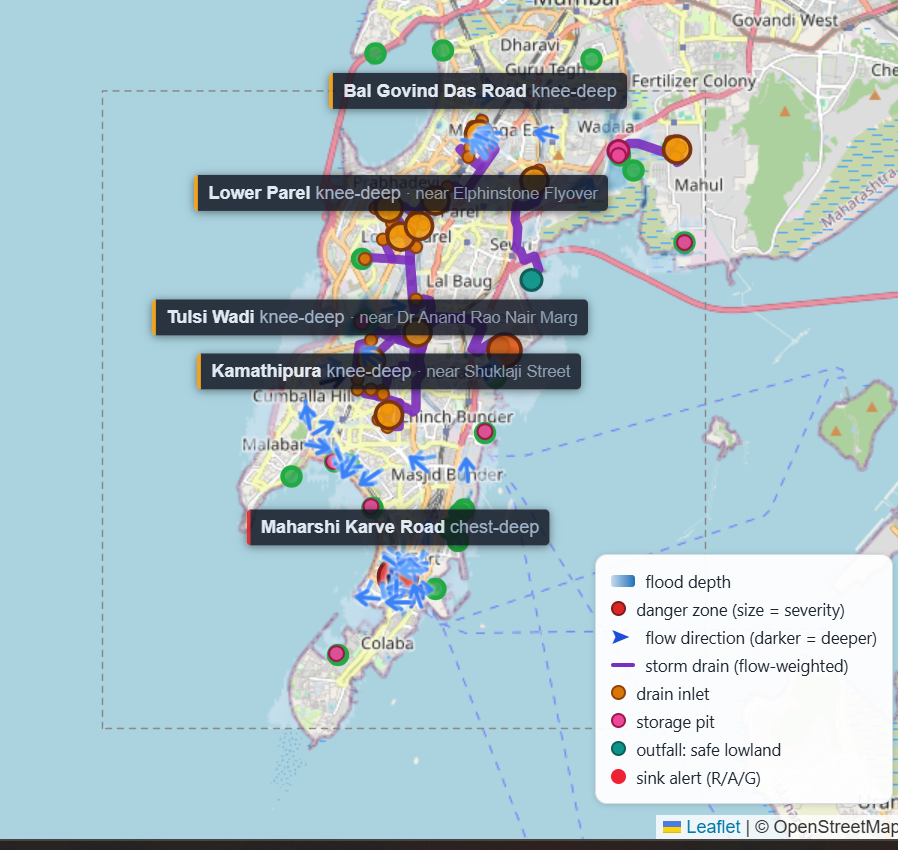
\includegraphics[width=0.99\linewidth]{figures/live_mumbai_city.png}\\[2pt]
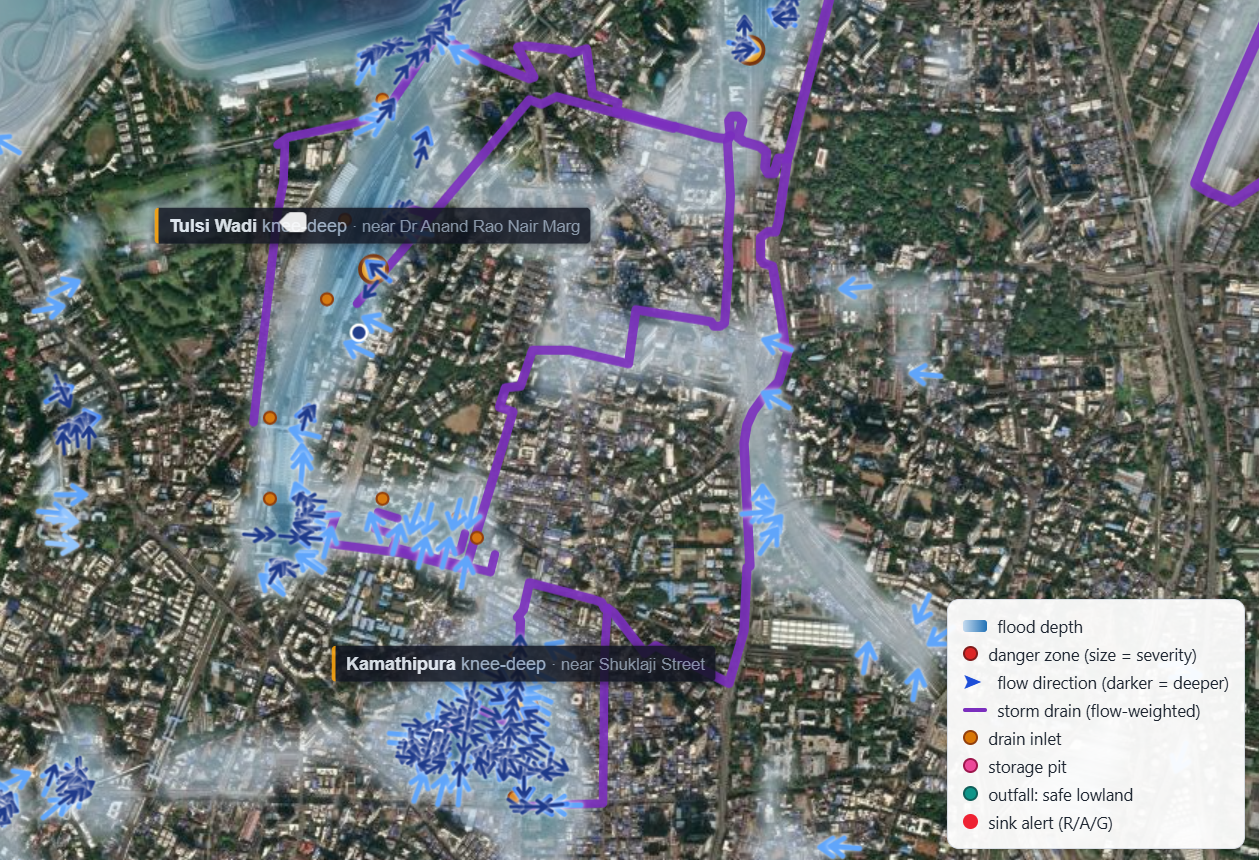
\includegraphics[width=0.99\linewidth]{figures/live_mumbai_sat.png}
\caption{Mumbai island city. \textbf{Top:} the planned network for the whole tile, with labelled
streets at knee and chest depth through Lower Parel, Kamathipura and Tulsi Wadi. Green circles are
safe-lowland outfalls and pink circles are storage pits. \textbf{Bottom:} the same plan over
satellite imagery. The trunks follow the street grid because that is where gravity and buildability
agree.}
\label{fig:mumbai}
\end{figure}

\subsection{Why we trust these decisions given Section~\ref{sec:dem}}
The quantities that drive the plans are the ones the elevation ensemble shows to be robust. Those
are total flooded volume, the existence of a basin, the approximate ordering of depths, and the
downhill topology. They are not the exact street that ponds first. The planner's outputs are also
portfolios, made of many inlets and many small basins, whose value degrades gracefully if any single
pond turns out to be somewhere else. We therefore frame the outputs as relative planning guidance,
meaning which strategy, at what density, and where to start, rather than as certified absolute
depths.
